\begin{example}
  [While Loop Example with Two Paths Iterating Alternatively]
  \label{ex:whileOdd}
  { \small
  \begin{figure}
  \centering
  \begin{subfigure}{.4\textwidth}
    \begin{centering}
    {\small
    $
    \begin{array}{l}
      \kw{whileOdd}(k) \triangleq \\
      \clabel{ \assign{i}{k} }^{0} ; \\
          \ewhile ~ \clabel{i > 0}^{1} ~ \edo ~ \\
          \qquad \Big(
            \eif(\clabel{i \% 2 = 0 }^{2},
            % \qquad \qquad 
            \clabel{\assign{i}{i - 1}}^{3},
            % \qquad \qquad 
            \clabel{\assign{i}{i - 3}}^{4});
            \Big)
      \end{array}
    $
    }
    \caption{}
    \end{centering}
    \end{subfigure}
  \begin{subfigure}{.5\textwidth}
    \begin{centering}
  %   \todo{abstract-cfg for two round}
  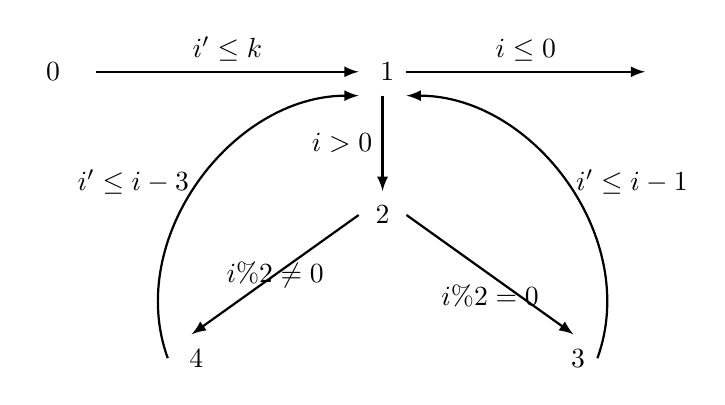
\begin{tikzpicture}[scale=\textwidth/20cm,samples=200]
  \draw[] (-7, 10) circle (0pt) node{{ $0$}};
  \draw[] (0, 10) circle (0pt) node{{ $1$}};
  \draw[] (0, 7) circle (0pt) node{\textbf{$2$}};
  \draw[] (4, 4) circle (0pt) node{{ $3$}};
  % \draw[] (0, 1) circle (0pt) node{{ $4$}};
  \draw[] (-4, 4) circle (0pt) node{{ $4$}};
  % Counter Variables
  \draw[] (6, 10) circle (0pt) node {\textbf{$\lex$}};
  % \draw[] (6, 4) circle (0pt) node {{ $ex$}};
  %
  % Control Flow Edges:
  \draw[ thick, -latex] (-6, 10)  -- node [above] {$i' \leq k$}(-0.5, 10);
  \draw[ thick, -latex] (0, 9.5)  -- node [left] {$i > 0$} (0, 7.5) ;
  \draw[ thick, -latex] (0.5, 7)  -- node [below] {$ i \% 2 = 0 $}  (4, 4.5);
  \draw[ thick, -latex] (-4.5, 4)  to  [out=110,in=180]  node [left] {$i' \leq i - 3$ }(-0.5, 9.5);
  \draw[ thick, -latex] (4.5, 4)  to  [out=70,in=0]   node [right] {$i' \leq i - 1$ }(0.5, 9.5);
  \draw[ thick, -latex]  (-0.5, 7) -- node  {$i \% 2 \neq 0$}  (-4, 4.5) ;
  \draw[ thick, -latex] (0.5, 10)  -- node [above] {$i \leq 0$}  (5.5, 10);
  % \draw[ thick, -latex] (6, 6.5)  -- node [right] {$\top$} (6, 4.5) ;
  \end{tikzpicture}
  \caption{}
    \end{centering}
    \end{subfigure}
  \caption{
  (a) The Simple While Loop Example with Two Paths Iterating Alternatively
    (b) The Abstract Execution Control Flow Graph}
      \label{fig:whileOdd}
  \end{figure}
  }
  %
  \end{example}    
  \begin{enumerate}
    \item  \textbf{The Abstract Execution Control Flow Graph} is generated in Figure~\ref{fig:whileOdd}(b).
    \item \textbf{Program Refinement}
    \\
    The loop free simple transition paths are computed as follows,
    \[
    \begin{array}{ll}
      \tpath_0 = (0 \to 1)
      &
      \tpath_1 = (1 \to 2), (2 \to 3), (3 \to 1)
      \\
      \tpath_2 = (1 \to 2), (2 \to 4), (4 \to 1)
      &
      \tpath_3 = (1 \to \lex)
    \end{array}
    \]
  \textbf{Refined Program}:
  \[
    \tpath_0 ; \rpchoose{1: \rprepeat(\tpath_1; \tpath_2) , 
    1: \rprepeat(\tpath_2; \tpath_1)}; \tpath_3
    \]
  \item \textbf{Outside-In Algorithm} : Compute Local Bound for Every program and sub programs.
  \[
    \begin{array}{lll}
      \outinB(\tpath_0) = 1
      &
      \outinB(\tpath_3) = 1
      &
      \outinB(\rprepeat(\tpath_1; \tpath_2)) = \frac{n}{4} 
      \\
      \outinB(\tpath_1) = 1 
      &
      \outinB(\tpath_2) = 1 
      &
      \outinB(\rprepeat(\tpath_2; \tpath_1)) = \frac{n}{4}
    \end{array}
    \]
  %       $\outinB(\tpath_0) = 1$
  % \\
  % $\outinB(\tpath_3) = 1$
  % \\
  % $\outinB(\tpath_1) = 1 $
  % \\
  % $\outinB(\rprepeat(\tpath_1; \tpath_2)) = \frac{n}{4} $
  % \\
  % $\outinB(\tpath_2) = 1 $
  % \\
  % $\outinB(\rprepeat(\tpath_2; \tpath_1)) = \frac{n}{4} $
  % \\
  % $\outinB(1: \rpchoose(\rprepeat_2(\cdots), \tpath_1)) 
  % = \max\{m, \frac{n}{m}\} $
  % \\
  \item \textbf{Inside-Out Algorithm}
  \begin{itemize}
    \item \textbf{Repeat Chain Set}
    \\
    $\rpchset(1, \tpath_1) = \{ \rprepeat(\tpath_1; \tpath_2) \to \tpath_1\}$ \\
    $\rpchset(1, \tpath_2) = \{ \rprepeat(\tpath_2; \tpath_1) \to \tpath_2\}$ \\
    $\rpchset(\_, \_) = \emptyset$ 
    % \\
    \item \textbf{Repeat Chain Bound} for every simple transition path $\tpath$ through its \emph{Repeat Chain}s
    $\rpchB(1, \tpath_1) = \frac{n}{4}$ \\
    $\rpchB(1, \tpath_2) = \frac{n}{4}$ 
    %
    \item \textbf{Loop Chain}
    \[
      % \begin{array}{ll}
        \lpch(\tpath_1) = 1 \to \tpath_1
        \quad
        \lpch(\tpath_2) = 1 \to \tpath_2
        \quad
        \lpch(\tpath_0) = \tpath_0
        \quad
        \lpch(\tpath_3) = \tpath_3
      % \end{array}
      \]
    % $\lpch(\tpath_1) = \{1\to \tpath_1\}$ \\
    % $\lpch(\tpath_2) = \{1\to \tpath_2\}$ \\
    % $\lpch(\tpath_0) = \{\tpath_0\}$ \\
    % $\lpch(\tpath_3) = \{\tpath_3\}$ 
    \item \textbf{{Relative Loop Bound}} for every simple transition path $\tpath$ through its \emph{Loop Chain}
    \[
    %   \begin{array}{ll}
        \rpchB(1, \tpath_1) = \frac{n}{4}
        \qquad
        \rpchB(1, \tpath_2) = \frac{n}{4}
        \qquad
        \rpchB(\bot, \tpath_0) = 1
        \qquad
        \rpchB(\bot, \tpath_3) = 1
      % \end{array}
      \]
    % $\rpchB(1, \tpath_1) = \frac{n}{4}$ \\
    % $\rpchB(1, \tpath_2) = \frac{n}{4}$  \\
    % $\rpchB(\bot, \tpath_0) = 1$ \\
    % $\rpchB(\bot, \tpath_3) = 1$ 
    \item \textbf{Path-Sensitive Reachability-Bound} for every simple transition path $\tpath$
    \\
    $\inoutB(\tpath_1) = \frac{n}{4}$ \quad
    $\inoutB(\tpath_2) = \frac{n}{4}$ \quad
    $\inoutB(\tpath_0) = 1$ \quad
    $\inoutB(\tpath_3) = 1$ 
  \end{itemize}
  \item \textbf{Path Sensitive Reachability-Bound} on every program control location
  \\
  $\psRB(\{0, \lex\}) = 1$ \quad
  $\psRB(\{3, 4 \}) = \lfloor \frac{n}{4} \rfloor$ \quad
  $\psRB(\{2, 1\}) = \lfloor \frac{n}{2} \rfloor + 1$ \quad
  \end{enumerate}